\documentclass[xcolor=x11names,compress]{beamer}

%% General document %%%%%%%%%%%%%%%%%%%%%%%%%%%%%%%%%%
\usepackage{graphicx}
\usepackage{mathpazo}
\usepackage[english]{babel}
\usepackage[T1]{fontenc}
\usepackage[utf8]{inputenc}
\usepackage{xcolor}
\usepackage{siunitx}
\usepackage{graphicx}
\usepackage{physics}
\usepackage{multimedia}
\usepackage[absolute,overlay]{textpos}
\usepackage{ragged2e}
\usepackage{amssymb}
\usepackage[version=4]{mhchem}
\usepackage[style=verbose,backend=bibtex]{biblatex}
\bibliography{SlideToulouse}



%%%%%%%%%%%%%%%%%%%%%%%%%%%%%%%%%%%%%%%%%%%%%%%%%%%%%%


%% Beamer Layout %%%%%%%%%%%%%%%%%%%%%%%%%%%%%%%%%%
\useoutertheme[subsection=false,shadow]{miniframes}
\useinnertheme{default}


\setbeamerfont{title like}{shape=\scshape}
\setbeamerfont{frametitle}{shape=\scshape}
\setbeamerfont{framesubtitle}{size=\normalsize}
\setbeamerfont{caption}{size=\scriptsize}
\setbeamercolor*{lower separation line head}{bg=DeepSkyBlue4} 
\setbeamercolor*{normal text}{fg=black,bg=white} 
\setbeamercolor*{alerted text}{fg=red} 
\setbeamercolor*{example text}{fg=black} 
\setbeamercolor*{structure}{fg=black} 

 
\setbeamercolor*{palette tertiary}{fg=black,bg=black!10} 
\setbeamercolor*{palette quaternary}{fg=black,bg=black!10} 
\setbeamercolor{caption name}{fg=DeepSkyBlue4}
\setbeamercolor{title}{fg=DeepSkyBlue4}
\setbeamercolor{itemize item}{fg=DeepSkyBlue4}
\setbeamercolor{frametitle}{fg=DeepSkyBlue4}
\renewcommand{\(}{\begin{columns}}
\renewcommand{\)}{\end{columns}}
\newcommand{\<}[1]{\begin{column}{#1}}
\renewcommand{\>}{\end{column}}
%%%%%%%%%%%%%%%%%%%%%%%%%%%%%%%%%%%%%%%%%%%%%%%%%%


\setbeamertemplate{navigation symbols}{} 
\setbeamertemplate{footline}[frame number]
\setbeamertemplate{caption}[numbered]
\setbeamertemplate{section in toc}[ball]
\setbeamertemplate{itemize items}[circle]
\beamerboxesdeclarecolorscheme{clair}{Coral4}{Ivory2}
\beamerboxesdeclarecolorscheme{foncé}{DarkSeaGreen4}{Ivory2}

\title[Title]{Perturbation theories in the complex plane}
\author[]{Antoine \textsc{Marie}}
  \setbeamersize{text margin left=5mm}
  \setbeamersize{text margin right=5mm}
\institute{Supervised by Pierre-François \textsc{LOOS}} 

\begin{document}




%%%%%%%%%%%%%%%%%%%%%%%%%%%%%%%%%%%%%%%%%%%%%%%%%%%%%%
%%%%%%%%%%%%%%%%%%%%%%%%%%%%%%%%%%%%%%%%%%%%%%%%%%%%%%

\begin{frame}[plain]

\date{30th June 2020}
\titlepage
\end{frame}

%%%%%%%%%%%%%%%%%%%%%%%%%%%%%%%%%%%%%%%%%%%%%%%%%%%%%%
%%%%%%%%%%%%%%%%%%%%%%%%%%%%%%%%%%%%%%%%%%%%%%%%%%%%%%

\begin{frame}{Why do we use perturbation theories in computational chemistry?}

\pause[1]

The Hartree-Fock theory is \textcolor{Green4}{computationally cheap} and can be applied even to \textcolor{Green4}{large systems}.

But this method is missing the \textcolor{red}{correlation energy}...

\vspace{0.5cm}

\pause[2]

$\rightarrow$ We need methods to get this correlation energy! 

\vspace{0.5cm}

\pause[3]

\begin{beamerboxesrounded}[scheme=foncé]{\centering A general method}
In physics perturbation theory is often a good way to improve the obtained results with an approximated Hamiltonian.
\end{beamerboxesrounded}

    
\end{frame}

\section{\textsc{Strange behaviors of the MP series}}

\begin{frame}{The Møller-Plesset perturbation theory}

\pause[1]

\begin{beamerboxesrounded}[scheme=foncé]{\centering Partitioning of the Hamiltonian}

\begin{equation}
   H = H_0 + \lambda V
\end{equation}

\end{beamerboxesrounded}

\begin{itemize}
\centering
    \item $H_0$: Unperturbed Hamiltonian
    \item $V$: Perturbation operator
\end{itemize}

\pause[2]

\begin{beamerboxesrounded}[scheme=foncé]{\centering The Fock operator}

\begin{equation}
   F = T + J + K
\end{equation}

\end{beamerboxesrounded}

\begin{itemize}
\centering
    \item $T$: Kinetic energy operator
    \item $J$: Coulomb operator
    \item $K$: Exchange operator
\end{itemize}

\pause[3]

\begin{beamerboxesrounded}[scheme=foncé]{}
\centering

Full Configuration Interaction gives access to high-order terms of the perturbation series!

\end{beamerboxesrounded}
    
\end{frame}

\begin{frame}{Deceptive or slow convergences\footcite{gill_deceptive_1986}}

\begin{figure}
    \centering

    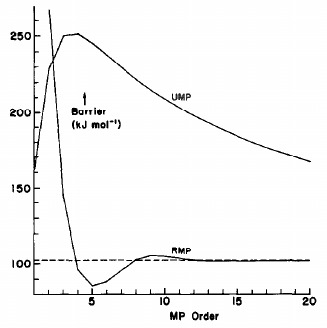
\includegraphics[width=0.45\textwidth]{gill1986.png}

    \caption{\centering Barriers to homolytic fission of \ce{He2^2+} at MPn/STO-3G level ($n = 1$--$20$).}
    \label{fig:my_label}
\end{figure}

    
\end{frame}

\begin{frame}{Multi-reference and spin contamination\footcite{gill_why_1988}}
\begin{table}
    \centering
    \begin{tabular}{c c c c c c c}
\hline
 $r$ & UHF & UMP2 & UMP3 & UMP4 & $\expval{S^2}$ \\
\hline
0.75 & 0.0\% & 63.8\% & 87.4\% & 95.9\% & 0.00\\
1.35 & 0.0\% & 15.2\% & 26.1\% & 34.9\% & 0.49\\
2.00 & 0.0\% & 01.0\% & 01.8\% & 02.6\% & 0.95\\
2.50 & 0.0\% & 00.1\% & 00.3\% & 00.4\% & 0.99\\
\hline
\end{tabular}
    \caption{\centering Percentage of electron correlation energy recovered and $\expval{S^2}$ for the \ce{H2} molecule as a function of bond length (r,\si{\angstrom}) in the STO-3G basis set.}
    \label{tab:my_label}
\end{table}

    
\end{frame}

\begin{frame}{Divergent cases}
  
\begin{figure}
    \centering
    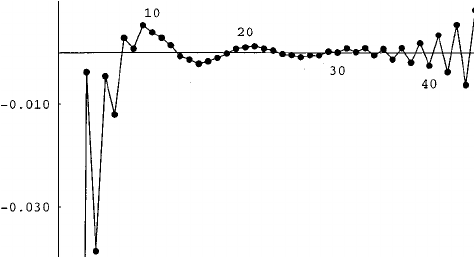
\includegraphics[width=0.6\textwidth]{The-energy-corrections-for-HF-at-stretched-geometry-in-the-cc-pVDZ-basis.png}
    \caption{The energy corrections for HF at stretched geometry in the cc-pVDZ basis. \footcite{olsen_divergence_2000}}
    \label{fig:my_label}
\end{figure}

\end{frame}

\section{The complex plane}

\begin{frame}{A simple example}

\begin{columns}

\column{0.48\textwidth}

\begin{beamerboxesrounded}[scheme=foncé]{An example function}

\begin{equation*}
   \frac{1}{1 + x^4}
\end{equation*}

\end{beamerboxesrounded}

\vspace{1cm}

\begin{itemize}
    \item Smooth for $x \in \mathbb{R}$
    
    \item Infinitely differentiable in $\mathbb{R}$
\end{itemize}

\column{0.48\textwidth}

    \begin{figure}
    \centering
    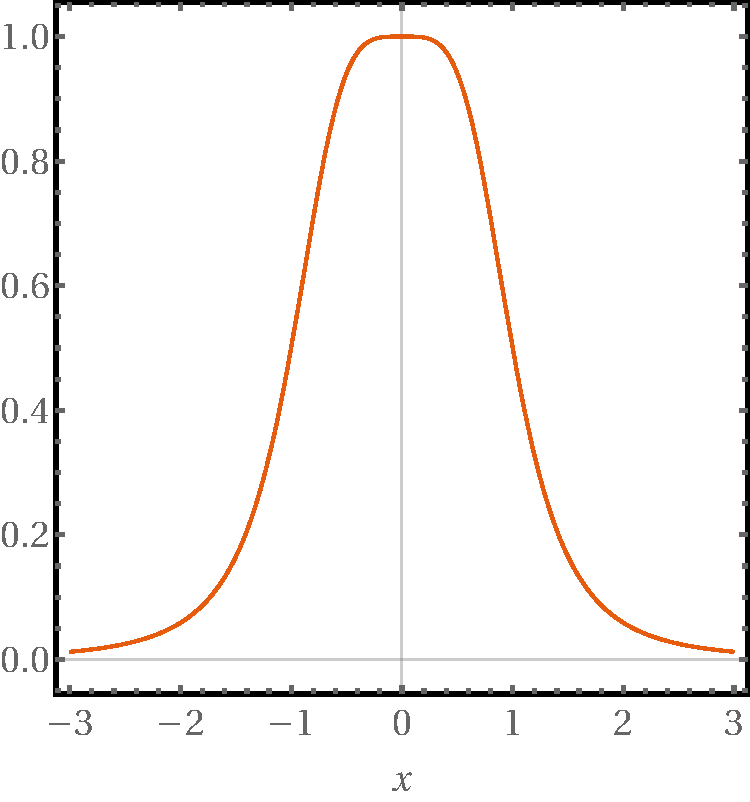
\includegraphics[width=0.6\textwidth]{exemplesingu.pdf}
    \caption{Plot of $1/(1+x^4)$}
    \label{fig:my_label}
\end{figure}

\end{columns}

But the Taylor expansion of this function does not converge for $x\geq1$... 
\vspace{0.3cm}
\centering Why ?

\end{frame}

\begin{frame}{And if we look in the complex plane?}

\begin{columns}

\column{0.48\textwidth}

\centering The function has 4 singularities in the complex plane!

\vspace{1cm}

$x = e^{i\pi/4}, e^{-i\pi/4}, e^{i3\pi/4}, e^{-i3\pi/4}$

\column{0.48\textwidth}

\begin{figure}
    \centering
    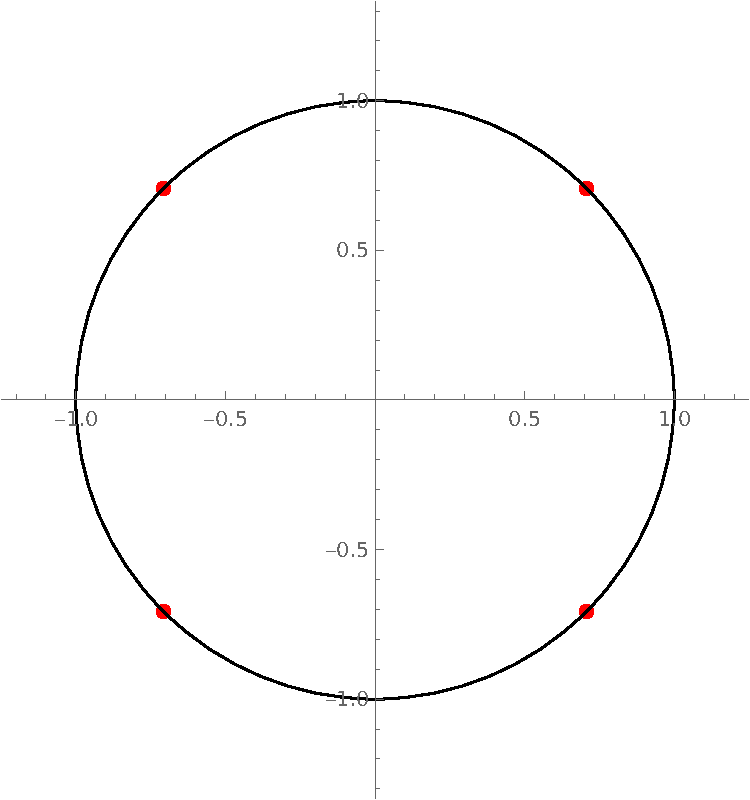
\includegraphics[width=0.6\textwidth]{possingu.pdf}
    \caption{\centering Singularities of the function $1/(1+x^4)$}
    \label{fig:my_label}
\end{figure}

\end{columns}

The \textcolor{red}{radius of convergence} of the Taylor expansion of a function is equal to the distance of the \textcolor{red}{closest singularity} to the origin in the \textcolor{red}{complex plane}.
    
\end{frame}

\begin{frame}{Extending chemistry in the complex plane}

\begin{beamerboxesrounded}[scheme=foncé]{\centering $\lambda$ a complex variable}

\begin{equation*}
   H(\lambda) = H_0 + \lambda V
\end{equation*}

\end{beamerboxesrounded}

\begin{columns}

\column{0.48\textwidth}

\begin{itemize}
    \item $n$ Riemann sheets
    \vspace{0.3cm}
    \item Exceptional points interconnecting the sheets
    \vspace{0.3cm}
    \item No ordering property in the complex plane
\end{itemize}

\column{0.48\textwidth}

\begin{figure}
    \centering
    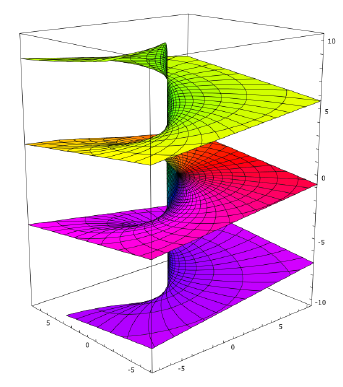
\includegraphics[width=0.7\textwidth]{riemannsheet.png}
    \label{fig:my_label}
\end{figure}

\end{columns}

\end{frame}

\section{Classifying the singularity}

\begin{frame}{Which features of the system localize the singularities?}

\begin{itemize}
    \item Partitioning of the Hamiltonian: Møller-Plesset, Epstein-Nesbet, \ldots
    \item Zeroth-order reference: weak or strong correlation.
    \item Finite or complete basis set.
    \item Localized or delocalized basis functions.
\end{itemize}
    
\end{frame}

\begin{frame}{A two-state model\footcite{olsen_divergence_2000}}

\begin{columns}

\column{0.48\textwidth}

\begin{figure}
    \centering
    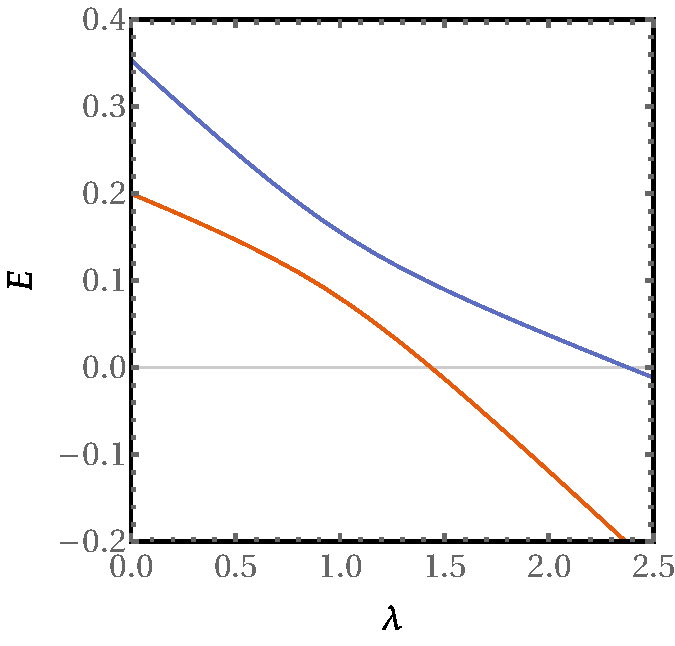
\includegraphics[width=0.8\textwidth]{avoidedcrossing.pdf}
    \caption{Example of an avoided crossing.}
    \label{fig:my_label}
\end{figure}

\column{0.48\textwidth}

\begin{beamerboxesrounded}[scheme=foncé]{A 2x2 matrix}
\centering \small{$\mqty(\alpha & \delta \\ \delta & \beta)  =$} 

\vspace{0.15cm}

\small{$\mqty(\alpha + \alpha_s & 0 \\ 0 & \beta + \beta_s ) + \mqty(- \alpha_s & \delta \\ \delta & - \beta_s)$}

\end{beamerboxesrounded}
\vspace{1cm}
\end{columns}
    
\end{frame}

\begin{frame}{Two-state model\footcite{olsen_divergence_2000}}
  
\begin{figure}
    \centering
    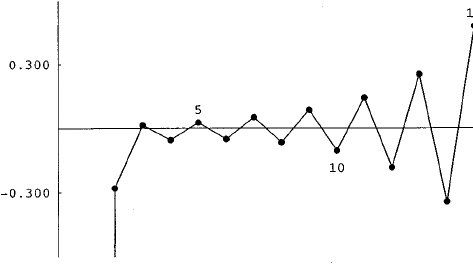
\includegraphics[width=0.6\textwidth]{figure-fig14.png}
    \caption{\centering The energy corrections for HF at stretched geometry in the aug'-cc-pVDZ basis with the two-state model.}
    \label{fig:my_label}
\end{figure}

\end{frame}

\begin{frame}{Existence of a critical point\footcite{stillinger_mollerplesset_2000}}

For $\lambda<0$:

\begin{equation*}
    H(\lambda)=\sum\limits_{j=1}^{2n}\left[ \underbrace{-\frac{1}{2}\grad_j^2 - \sum\limits_{k=1}^{N} \frac{Z_k}{|\vb{r}_j-\vb{R}_k|}}_{\text{Independant of }\lambda} + \overbrace{(1-\lambda)V_j^{(scf)}}^{\textcolor{red}{Repulsive}}+\underbrace{\lambda\sum\limits_{j<l}^{2n}\frac{1}{|\vb{r}_j-\vb{r}_l|}}_{\textcolor{blue}{Attractive}}  \right]
\end{equation*}

\end{frame}

\begin{frame}{Critical point in a finite basis set}

\pause[1]
    
\begin{beamerboxesrounded}[scheme=foncé]{\centering Exact energy $E(z)$}
$E(z)$ has a critical point on the negative real axis and $E(z)$ is continue for real values below $z_{crit}$.
\end{beamerboxesrounded}

\vspace{0.5cm}

\pause[2]

\begin{beamerboxesrounded}[scheme=foncé]{\centering In a finite basis set}
The singularities occur in complex conjugate pairs with non-zero imaginary parts and the energies are discrete. 
\end{beamerboxesrounded}

\vspace{0.5cm}

\pause[3]

\centering \Large{How is this connected???}
    
\end{frame}

\begin{frame}{Singularities $\alpha$ and $\beta$ \footcite{sergeev_singularities_2006}}

\pause[1]

\begin{beamerboxesrounded}[scheme=foncé]{\centering Observation}
We can separate singularities in two parts. 
\end{beamerboxesrounded}   

\pause[2]

\begin{beamerboxesrounded}[scheme=foncé]{\centering Singularity $\alpha$}
\begin{itemize}
    \item Large avoided crossing
    \item Non-zero imaginary part
    \item Interaction with a low-lying doubly excited states
\end{itemize} 
\end{beamerboxesrounded}  

\pause[3]

\begin{beamerboxesrounded}[scheme=foncé]{\centering Singularity $\beta$}
\begin{itemize}
    \item Sharp avoided crossing
    \item Very small imaginary part
    \item Interaction with a diffuse function 
\end{itemize} 
\end{beamerboxesrounded} 

\end{frame}



\begin{frame}{Modeling the critical point}

\pause[1]

\begin{beamerboxesrounded}[scheme=foncé]{\centering Stillinger}
\begin{quote}
    \textit{"One might expect that $E_{FCI}(z) $ would try to model a continuum at $z_c$ with a grouping of discrete but closely spaced eigenstates that undergo sharp avoided crossing with the ground states."}
\end{quote}
\end{beamerboxesrounded}

\vspace{0.5cm}

\pause[2]

\begin{beamerboxesrounded}[scheme=foncé]{\centering Sergeev et al.}
Proof of the existence of this group of sharp avoided crossings for Ne, He and HF when the basis set contains diffuse functions.
\end{beamerboxesrounded}
    
\end{frame}

\section{The spherium model}

\begin{frame}{Spherium: a theoretical playground\footcite{loos_ground_2009}}

\begin{beamerboxesrounded}[scheme=foncé]{\centering Two electrons on a sphere Hamiltonian}
\begin{equation*}
    H=-\frac{1}{2}(\grad_1^2 + \grad_2^2) + \frac{1}{r_{12}}
\end{equation*} 
\end{beamerboxesrounded}
\vspace{0.5cm}

\begin{columns}

\column{0.48\textwidth}

\centering{Small $R$}
\vspace{0.5cm}

\begin{itemize}
    \item $E_\text{kin} \gg E_\text{pot}$
    \item Uniform density of electrons
    \item \textcolor{red}{Weak correlation}
\end{itemize}

\vspace{0.5cm}

\column{0.48\textwidth}

\centering{Large $R$}
\vspace{0.5cm}

\begin{itemize}
    \item $E_\text{kin} \ll E_\text{pot}$
    \item Electrons on the opposite sides of the sphere
    \item \textcolor{red}{Strong correlation}
    \end{itemize}

\end{columns}

\end{frame}

\begin{frame}{Apparition of a class $\beta$ singularity}

\pause[1]

\begin{beamerboxesrounded}[scheme=foncé]{\centering Expectation}
The electrons are restricted to the surface of the sphere so we should not observe singularities characteristic of ionization processes.
\end{beamerboxesrounded}

\vspace{0.5cm}

\pause[2]

\large But for some values of R... we actually observe some $\beta$ singularities!
\centering Why?

\vspace{0.5cm}

\pause[3]

\begin{beamerboxesrounded}[scheme=foncé]{\centering Symmetry breaking}
The $\beta$ singularities observed are connected to the symmetry breaking of the wave function.
\end{beamerboxesrounded}

\end{frame}

\begin{frame}{Conclusion}

\pause[1]

\begin{beamerboxesrounded}[scheme=foncé]{\centering Møller-Plesset perturbation theory}
By understanding how the singularities are localized in the complex plane we hope that it will gives us a deep understanding of the strengths and weaknesses of the Møller-Plesset method to get the correlation energy.
\end{beamerboxesrounded}

\pause[2]

\vspace{0.5cm}

But there is an other secret application of exceptional points...

\pause[3]

\vspace{0.5cm}

\begin{beamerboxesrounded}[scheme=foncé]{\centering A new way to excited states energies}
The exceptionnal points connect ground and excited states in the complex plane. Using those properties one can smoothly morph a ground state in an excited state. 
\end{beamerboxesrounded}
    
\end{frame}

\end{document}
